\documentclass[12pt,a4paper]{article}

% ==== PACKAGES ====
\usepackage[utf8]{inputenc}
\usepackage[T1]{fontenc}
\usepackage[english]{babel}
\usepackage{graphicx}
\usepackage{setspace}
\usepackage{geometry}
\geometry{margin=1in}
\usepackage{titling}
\usepackage{lmodern}
\usepackage{float}
\usepackage{caption}
\usepackage{listings}
\usepackage{xcolor}
\usepackage{url}

\lstdefinestyle{codestyle}{
  backgroundcolor=\color{gray!10}, 
  frame=single,                    
  rulecolor=\color{gray!70},       
  basicstyle=\ttfamily\small,      
  keywordstyle=\color{blue!70!black},
  commentstyle=\color{gray!60},
  stringstyle=\color{orange!90!black},
  showstringspaces=false,
  breaklines=true,
  tabsize=2
}
\setlength{\parindent}{0pt}
% ==== DOCUMENT ====
\begin{document}

% ==== TITLE PAGE ====
\begin{titlepage}
    \centering
    \vspace*{2cm}
    
    {\Huge \textbf{Workshop No. 3 - Backend Implementation and Testing}}\\[1.2cm]
    {\LARGE \textbf{Software Engineering Seminar}}\\[0.5cm]
    {\Large \textbf{Universidad Distrital Francisco José de Caldas}}\\[0.2cm]
    {\large \textbf{Systems Engineering Program}}\\[2cm]

    % Optional logo (remove comment if you have a logo)
    % \includegraphics[width=0.25\textwidth]{logo_ud.png}\\[1.5cm]

    {\Large \textbf{Presented by:}}\\[0.5cm]
    {\large Brayan Alejandro Riveros Rodríguez \\ \textit{20201020084}}\\[0.3cm]
    {\large Carlos Andrés Pescador Castro \\ \textit{20182020139}}\\[0.3cm]
    {\large Cristian Santiago Ríos Vásquez \\ \textit{20201020107}}\\[2cm]

    {\Large Bogotá D.C., Colombia}\\[0.3cm]
    {\large November 8, 2025}
    
    \vfill
\end{titlepage}

% ==== CONTENT ====

\section{Database Connection Scripts and Configuration}

\subsection{Overview}
The authentication backend for the \textbf{Course Finder System} uses a MySQL 8 database for secure storage of administrator credentials. 
The connection between the Spring Boot backend and the database is managed via \texttt{Spring Data JPA} and configured in the 
\texttt{application.properties} file.

\subsection{Database Initialization Script}
The database schema is initialized through the SQL script located at \url{init_db_scripts/schema_db.sql}. \\ 

This script ensures that the database and required tables are properly created during setup.  \\

\begin{lstlisting}[style=codestyle, language=SQL, caption={Database initialization script.}]
-- Database initialization script for auth-back
-- Database: auth_db_course

CREATE DATABASE IF NOT EXISTS auth_db_course 
  CHARACTER SET utf8mb4 
  COLLATE utf8mb4_unicode_ci;
USE auth_db_course;

DROP TABLE IF EXISTS admins;

CREATE TABLE admins (
    id INT AUTO_INCREMENT PRIMARY KEY,
    username VARCHAR(255) NOT NULL UNIQUE,
    password_hash VARCHAR(255) NOT NULL,
    email VARCHAR(255) NOT NULL UNIQUE,
    created_at TIMESTAMP DEFAULT CURRENT_TIMESTAMP,
    updated_at TIMESTAMP DEFAULT CURRENT_TIMESTAMP 
      ON UPDATE CURRENT_TIMESTAMP,
    INDEX idx_username (username),
    INDEX idx_email (email)
) ENGINE=InnoDB DEFAULT CHARSET=utf8mb4 
  COLLATE=utf8mb4_unicode_ci;
\end{lstlisting}


\subsection{Connection Configuration}
The connection to MySQL is configured within the \texttt{application.properties} file as follows:

\begin{lstlisting}[style=codestyle, language=Java, caption={Spring Boot MySQL configuration.}]
spring.datasource.url=jdbc:mysql://localhost:3306/auth_db_course?useSSL=false&serverTimezone=UTC
spring.datasource.username=root
spring.datasource.password=YOUR_PASSWORD
spring.datasource.driver-class-name=com.mysql.cj.jdbc.Driver

spring.jpa.hibernate.ddl-auto=update
spring.jpa.show-sql=true
spring.jpa.properties.hibernate.dialect=org.hibernate.dialect.MySQL8Dialect
server.port=8080
\end{lstlisting}


\textbf{Note:} Replace \texttt{YOUR\_PASSWORD} with your local MySQL credentials.

\subsection{Testing the Connection}
Once configured, the connection can be tested by running:

\begin{verbatim}
mvn spring-boot:run
\end{verbatim}

A successful connection will output:

\begin{verbatim}
Tomcat initialized with port 8080 (http)
Started AuthBackApplication in 3.2 seconds
\end{verbatim}

\section{REST API Documentation}

\subsection{Overview}
The backend exposes a REST API that provides authentication features for the Course Finder System.
All endpoints are fully documented using \textbf{Swagger UI}, which is automatically generated when the application starts.

\subsection{Accessing Swagger UI}
Once the application is running, the API documentation is available at:

\begin{center}
\texttt{http://localhost:8080/swagger-ui/index.html}
\end{center}

Swagger UI provides:
\begin{itemize}
    \item Interactive exploration of available endpoints.
    \item The ability to send test requests directly from the browser.
    \item Visualization of request and response formats, headers, and status codes.
\end{itemize}

\begin{figure}[H]
    \centering
    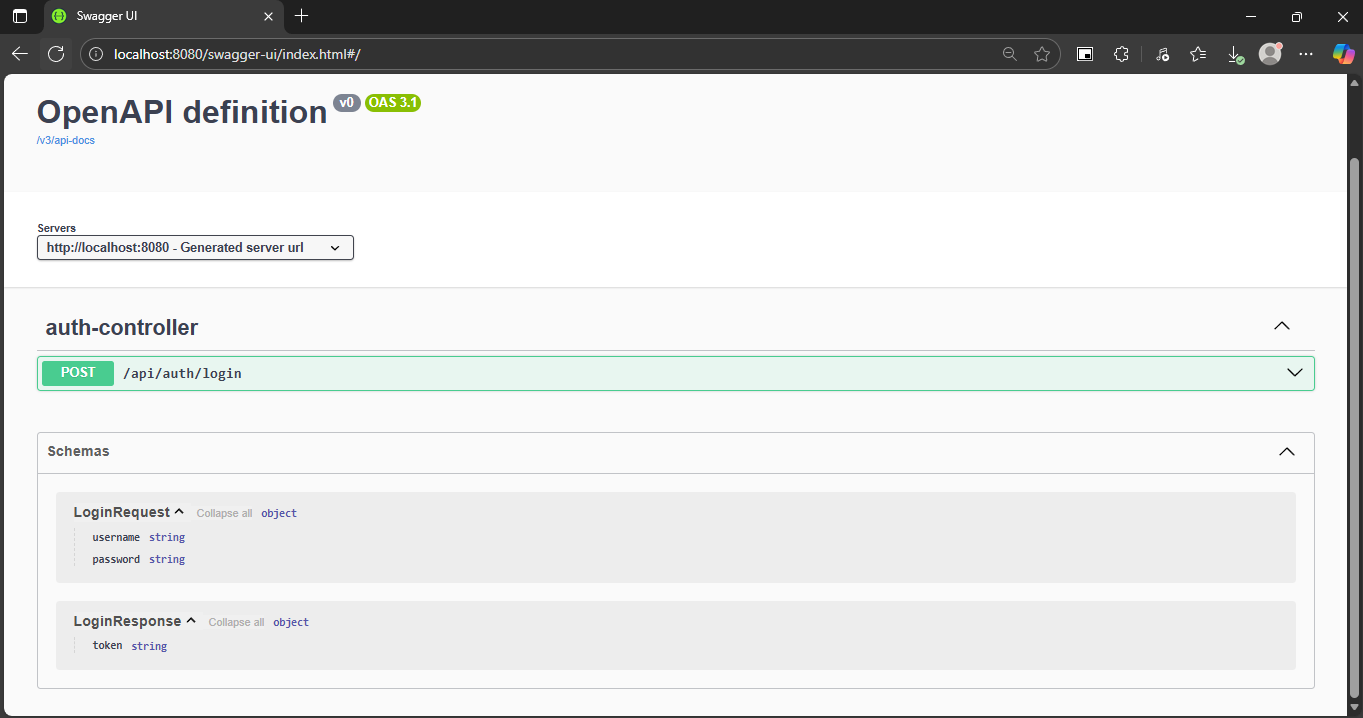
\includegraphics[width=0.9\linewidth]{media/Swagger.png}
    \caption{Swagger UI interface showing REST API endpoints.}
\end{figure}

\subsection{Authentication Endpoint}

\begin{table}[H]
\centering
\begin{tabular}{|l|l|l|}
\hline
\textbf{Method} & \textbf{Endpoint} & \textbf{Description} \\
\hline
POST & /api/auth/login & Authenticates an admin and returns a JWT token. \\
\hline
\end{tabular}
\caption{Main REST API endpoint.}
\end{table}

This endpoint handles administrator authentication within the system. 
It validates the provided username and password against the database and, if successful, 
generates a secure \textbf{JWT (JSON Web Token)} signed with the server’s private key. 
The token can then be used in subsequent requests to access protected resources.

\begin{figure}[H]
    \centering
    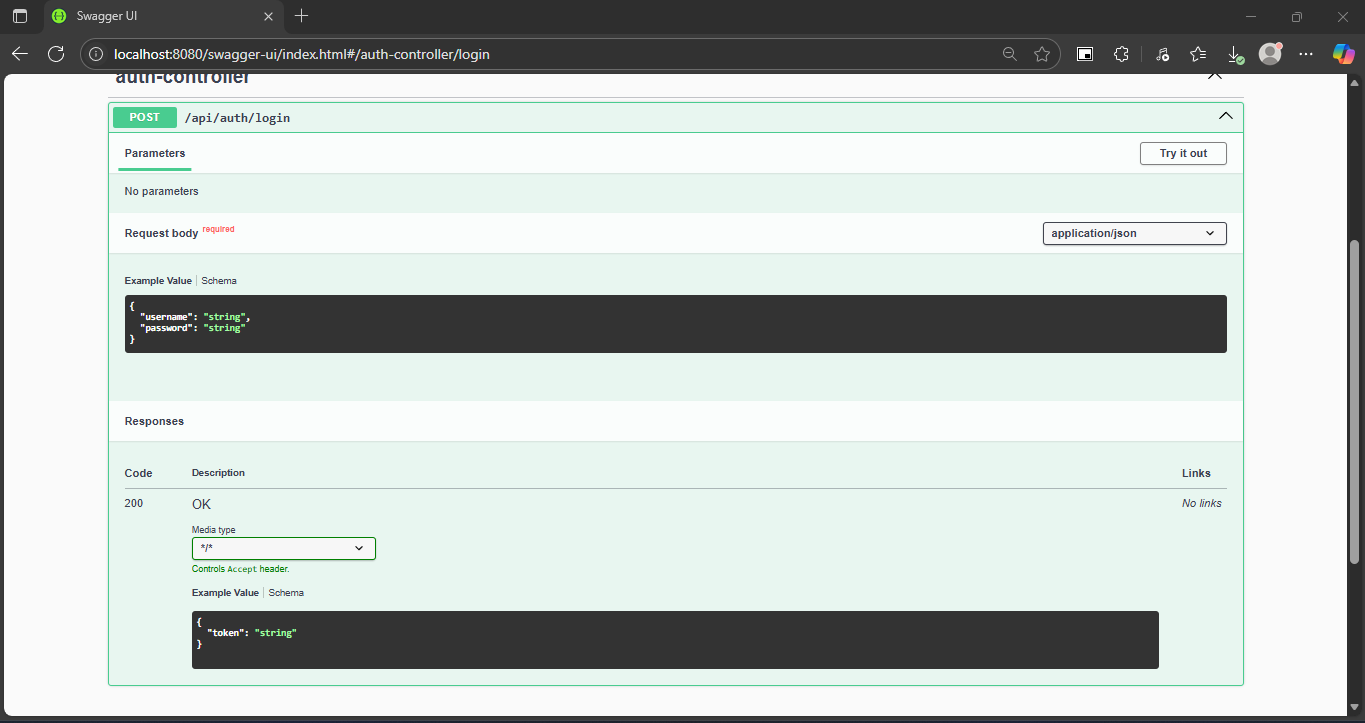
\includegraphics[width=0.85\linewidth]{media/LoginEndPoint.png}
    \caption{Authentication endpoint displayed in Swagger UI.}
\end{figure}

\textbf{Example request:}
\begin{verbatim}
{
  "username": "admin",
  "password": "admin123"
}
\end{verbatim}

\textbf{Example response:}
\begin{verbatim}
{
  "token": "eyJhbGciOiJIUzI1NiIsInR5..."
}
\end{verbatim}

\begin{figure}[H]
    \centering
    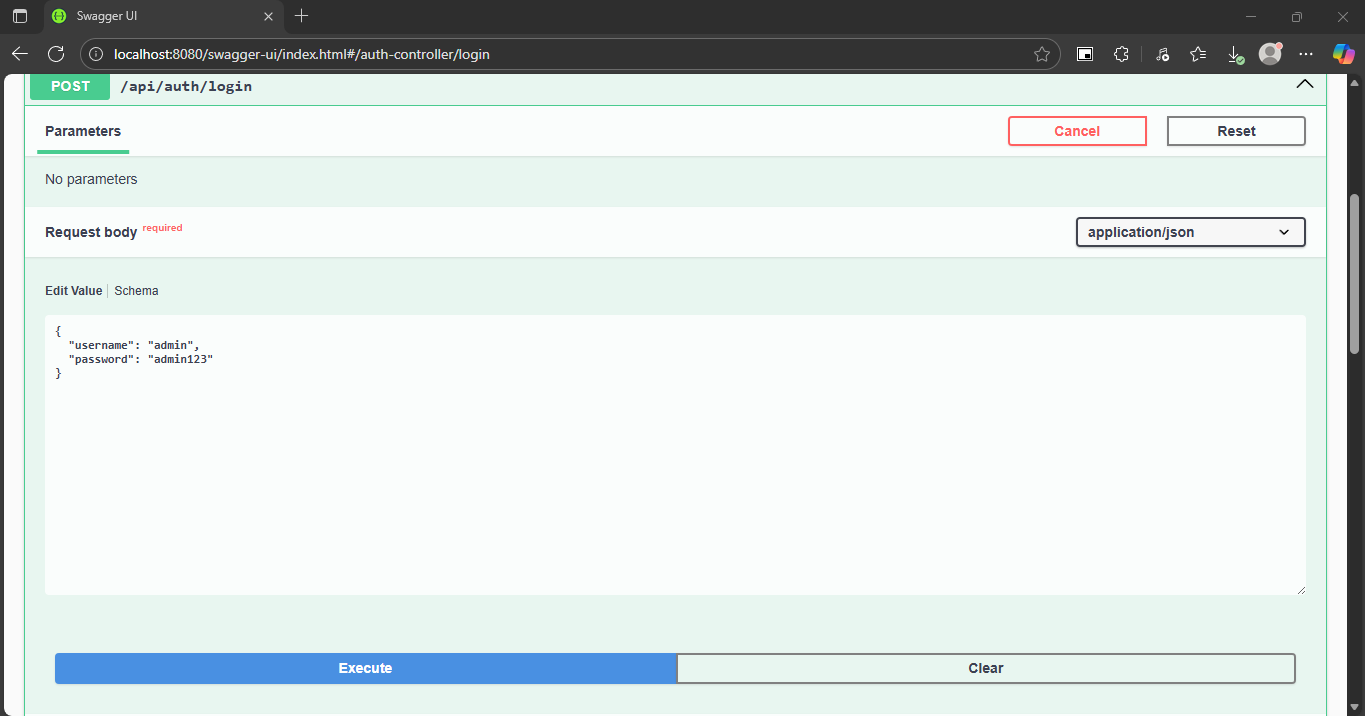
\includegraphics[width=0.85\linewidth]{media/TestG1.png}
    \caption{Example request executed from Swagger UI interface.}
\end{figure}

\begin{figure}[H]
    \centering
    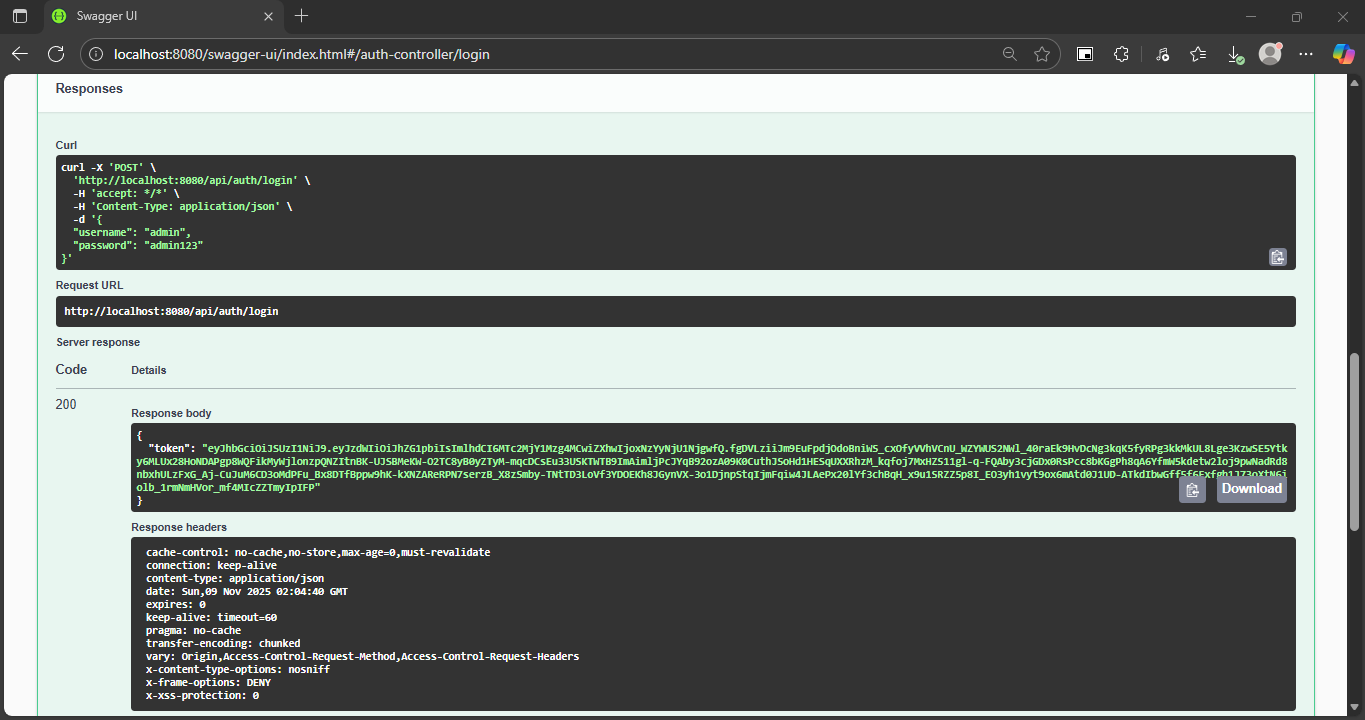
\includegraphics[width=0.85\linewidth]{media/TestG2.png}
    \caption{Example of a successful response returning a JWT token.}
\end{figure}



\section{Unit Test Results and Code}

\subsection{Overview}
Unit tests were implemented using \textbf{JUnit 5} and \textbf{Mockito} to validate the authentication logic and the generation of JWT tokens.  \\ 
\\
Tests are located in the \texttt{src/test/java/com/udistrital/authback/} directory.

\subsection{AuthServiceTest}
The \texttt{AuthServiceTest} class validates login logic, ensuring the authentication process behaves as expected.

\begin{itemize}
    \item \textbf{Successful login:} Verifies that valid credentials return a JWT token.
    \item \textbf{Invalid password:} Ensures wrong credentials raise an exception.
    \item \textbf{User not found:} Confirms proper handling of missing user entries.
\end{itemize}

\begin{figure}[H]
    \centering
    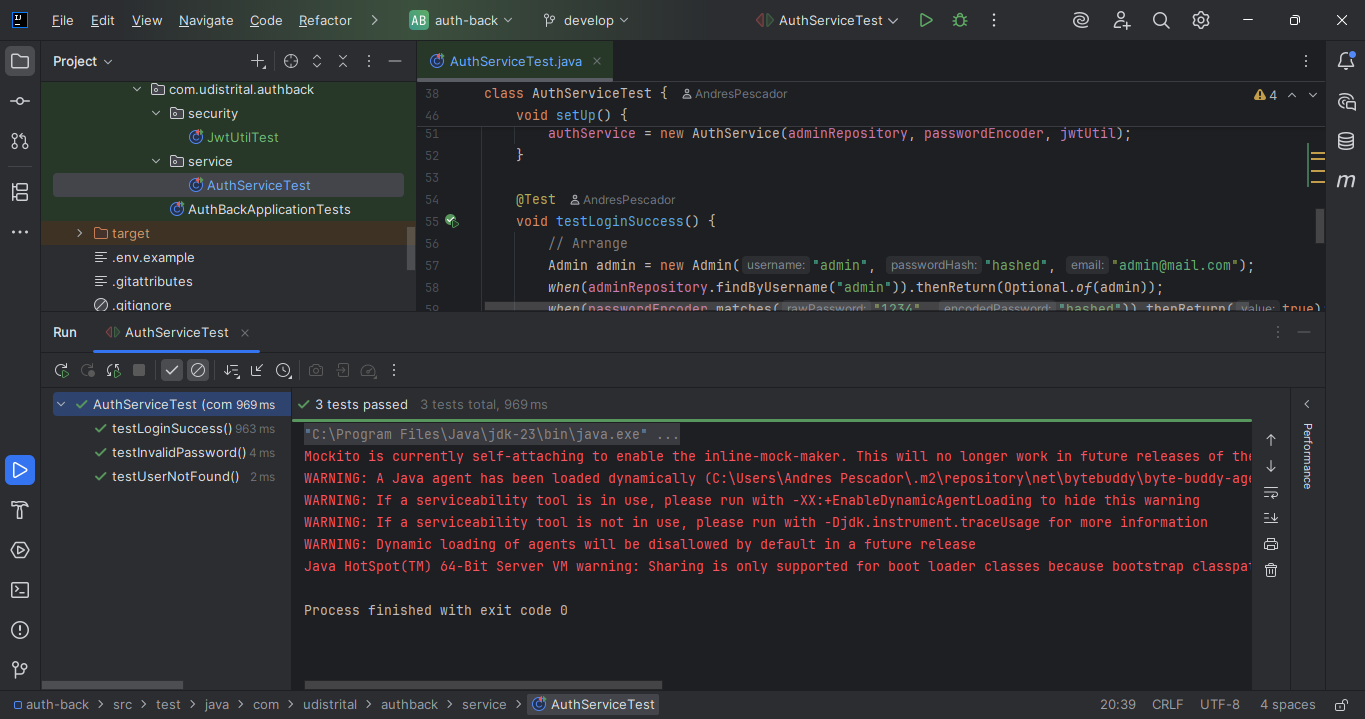
\includegraphics[width=0.85\linewidth]{media/UnitTestAuthService.png}
    \caption{Successful execution of AuthService unit tests.}
\end{figure}

\subsection{JwtUtilTest}
The \texttt{JwtUtilTest} class tests the generation and signing of JWT tokens.

\begin{itemize}
    \item \textbf{Token generation:} Validates that the token includes correct claims.
    \item \textbf{Signature verification:} Confirms the private key correctly signs tokens using RS256.
    \item \textbf{Expiration:} Checks that the token expiration time is applied correctly.
\end{itemize}

\begin{figure}[H]
    \centering
    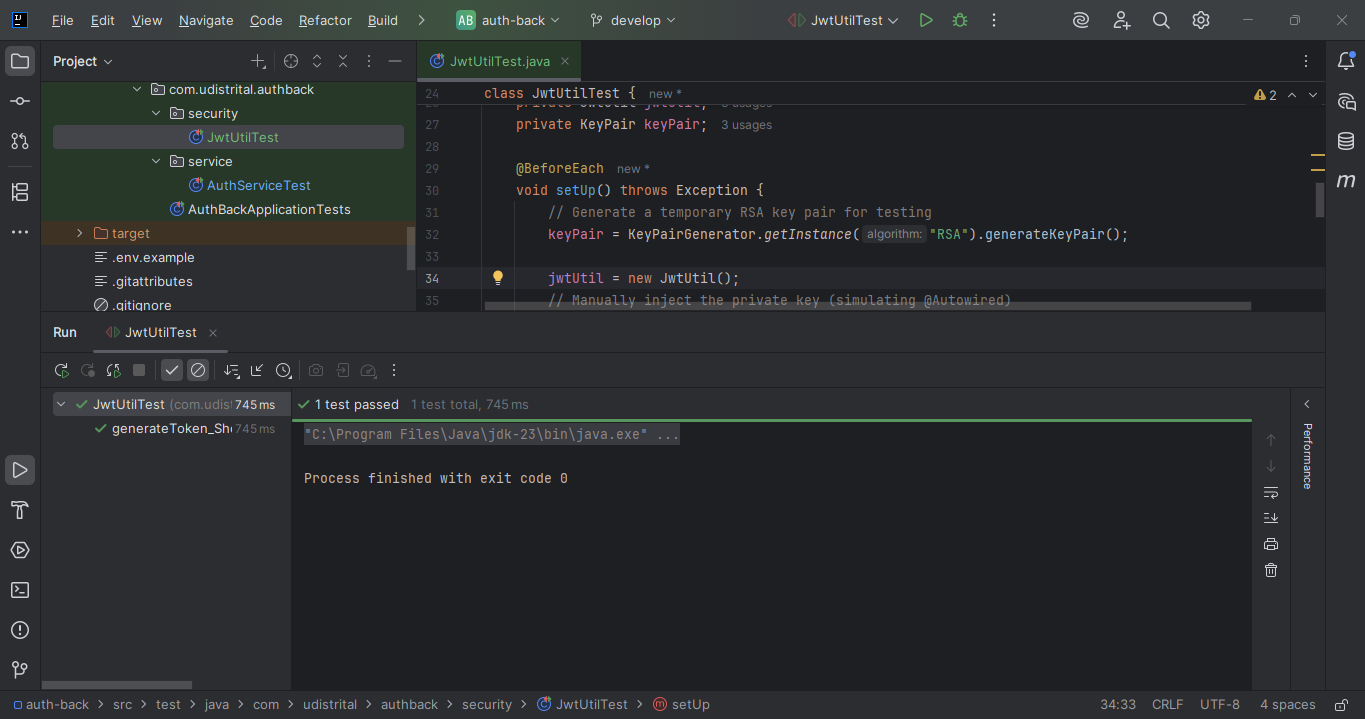
\includegraphics[width=0.85\linewidth]{media/UnitTestJWTUtil.png}
    \caption{Successful execution of JwtUtil unit tests.}
\end{figure}

\subsection{Command to Run Tests}
All unit tests can be executed using the Maven command:
\begin{verbatim}
mvn test
\end{verbatim}

Example console output
\begin{verbatim}
Tests run: 4, Failures: 0, Errors: 0, Skipped: 0
BUILD SUCCESS
\end{verbatim}


\section{Conclusion}
This backend successfully integrates a secure MySQL connection, JWT-based authentication, and verified functionality through comprehensive unit testing. Swagger UI ensures clear API documentation and facilitates testing for both developers and system administrators.

\end{document}